
\subsection{GMAP, Plotting epicentres with Google maps or Google Earth} 
\label{subs:gmap}

%\textcolor{red}{jh-change:  peter: you name shoudl be removed everywhere in text sine you are now a coauthor. in gmap section describe browser used since firefox is harwired in eev, what if people use another ?}\newline
%\textcolor{green}{pv-change: firefox is nolonger hardwired in eev.}\newline
Google maps and Google Earth seem to quickly establish themselves as 
commonly used mapping tools. GMAP provides the conversion from Nordic 
format (s-files) to the input format required by these systems, 
which is the Keyhole Markup Language (KML). 
GMAP also convert SEISAN station and polygon files.
\index{Gmap}
\index{Google Earth}
\index{Google map} 
The input format of 
Google Earth is described on \url{http://earth.google.com/kml/}. 
GMAP required Google Earth installed on your system to plot 
the output file. Download Google Earth here 
\url{http://earth.google.com/download-earth.html} 
(note the terms and conditions on 
\url{http://pack.google.com/intl/en/eula\_print\_us.html}). 
To change the color codes se e.g. \url{http://html-color-codes.info/}.

% \href{http://earth.google.com/download-earth.html}{TEST}

GMAP can run in three modes: 
\begin{itemize}
\item The simple GMAP - runs in the browser with Google Map
\item The advanced GMAP - runs in the desktop version of Google Earth
\item The automatic GMAP - runs in the desktop version of Google Earth
\end{itemize}
The three modes are described below.

\subsubsection{The simple GMAP}
\index{GMAP simple} 
Type gmap in eev, a file \texttt{gmap.html} is created and copied to you 
GMAP\_DIR directory. When you open the \texttt{gmap.html} with your 
browser, you will be redirected to Google Maps and a green arrow will 
show the epicentre. The following parameters in \texttt{SEISAN.DEF} are used:
GMAP\_DIR /home/seismo/www\newline
GMAP\_TYPE MAP [MAP, SATELLITE, HYBRID or TERRAIN]\newline
GMAP\_TYPE determines which type of map Google MAPS will use, 
you can choose between: MAP, SATELLITE, HYBRID and TERRAIN. 

\subsubsection{The advanced GMAP}
\index{GMAP advanced} 
This mode of GMAP is a command line version, that convert SEISAN s-files to input 
files for Google Earth. It also convert SEISAN STATIONx.HYP files and polygone files.

\begin{itemize}
\item
Type \texttt{gmap} on the command line to start gmap.
\item
Type \texttt{gmap -help} to see the options. 
\item
Type \texttt{gmap -stat} to convert a SEISAN station files to kml. 
\item
Type \texttt{gmap -poly} to convert a SEISAN polygon files to kml. 
\end{itemize}

In \texttt{gmap} you can:
\begin{enumerate}
\item 
Set the colour of the icons. 
\item Show the error ellipse.
\item Show events as a animation over time. 
\item Set the scale of the icons (default: scale=0.2*mag**0.5). 
\item Set the type of icon used for earthquakes, explosions, probable explosions and for other events. 
\item Include or exclude the S-file. 
\item Rename the output file. 
\item Append text in KML format to the output file (See \texttt{SEISAN.DEF} parameters below). 
\end{enumerate}


Example: \newline
\begin{enumerate}
\item 
Use select to grap data from your Seisan database. 
\item Run the GMAP program:\newline
\begin{verbatim}
unix:/home/seismo/WOR: gmap 
 INPUT FILE NAME 
select.out 
Title: 
West Greenland [2000;2008]

Number of Earthquakes : 945 Explosions : 0 Probable Explosions : 2 Other events : 2 
Output file is
gmap.kml
\end{verbatim}

\item
In Google Earth open the output file gmap.kml. See Fig. \ref{fig:gmap}. 
\end{enumerate}

\begin{figure}
\htmlimage{scale=2.0}
\centerline{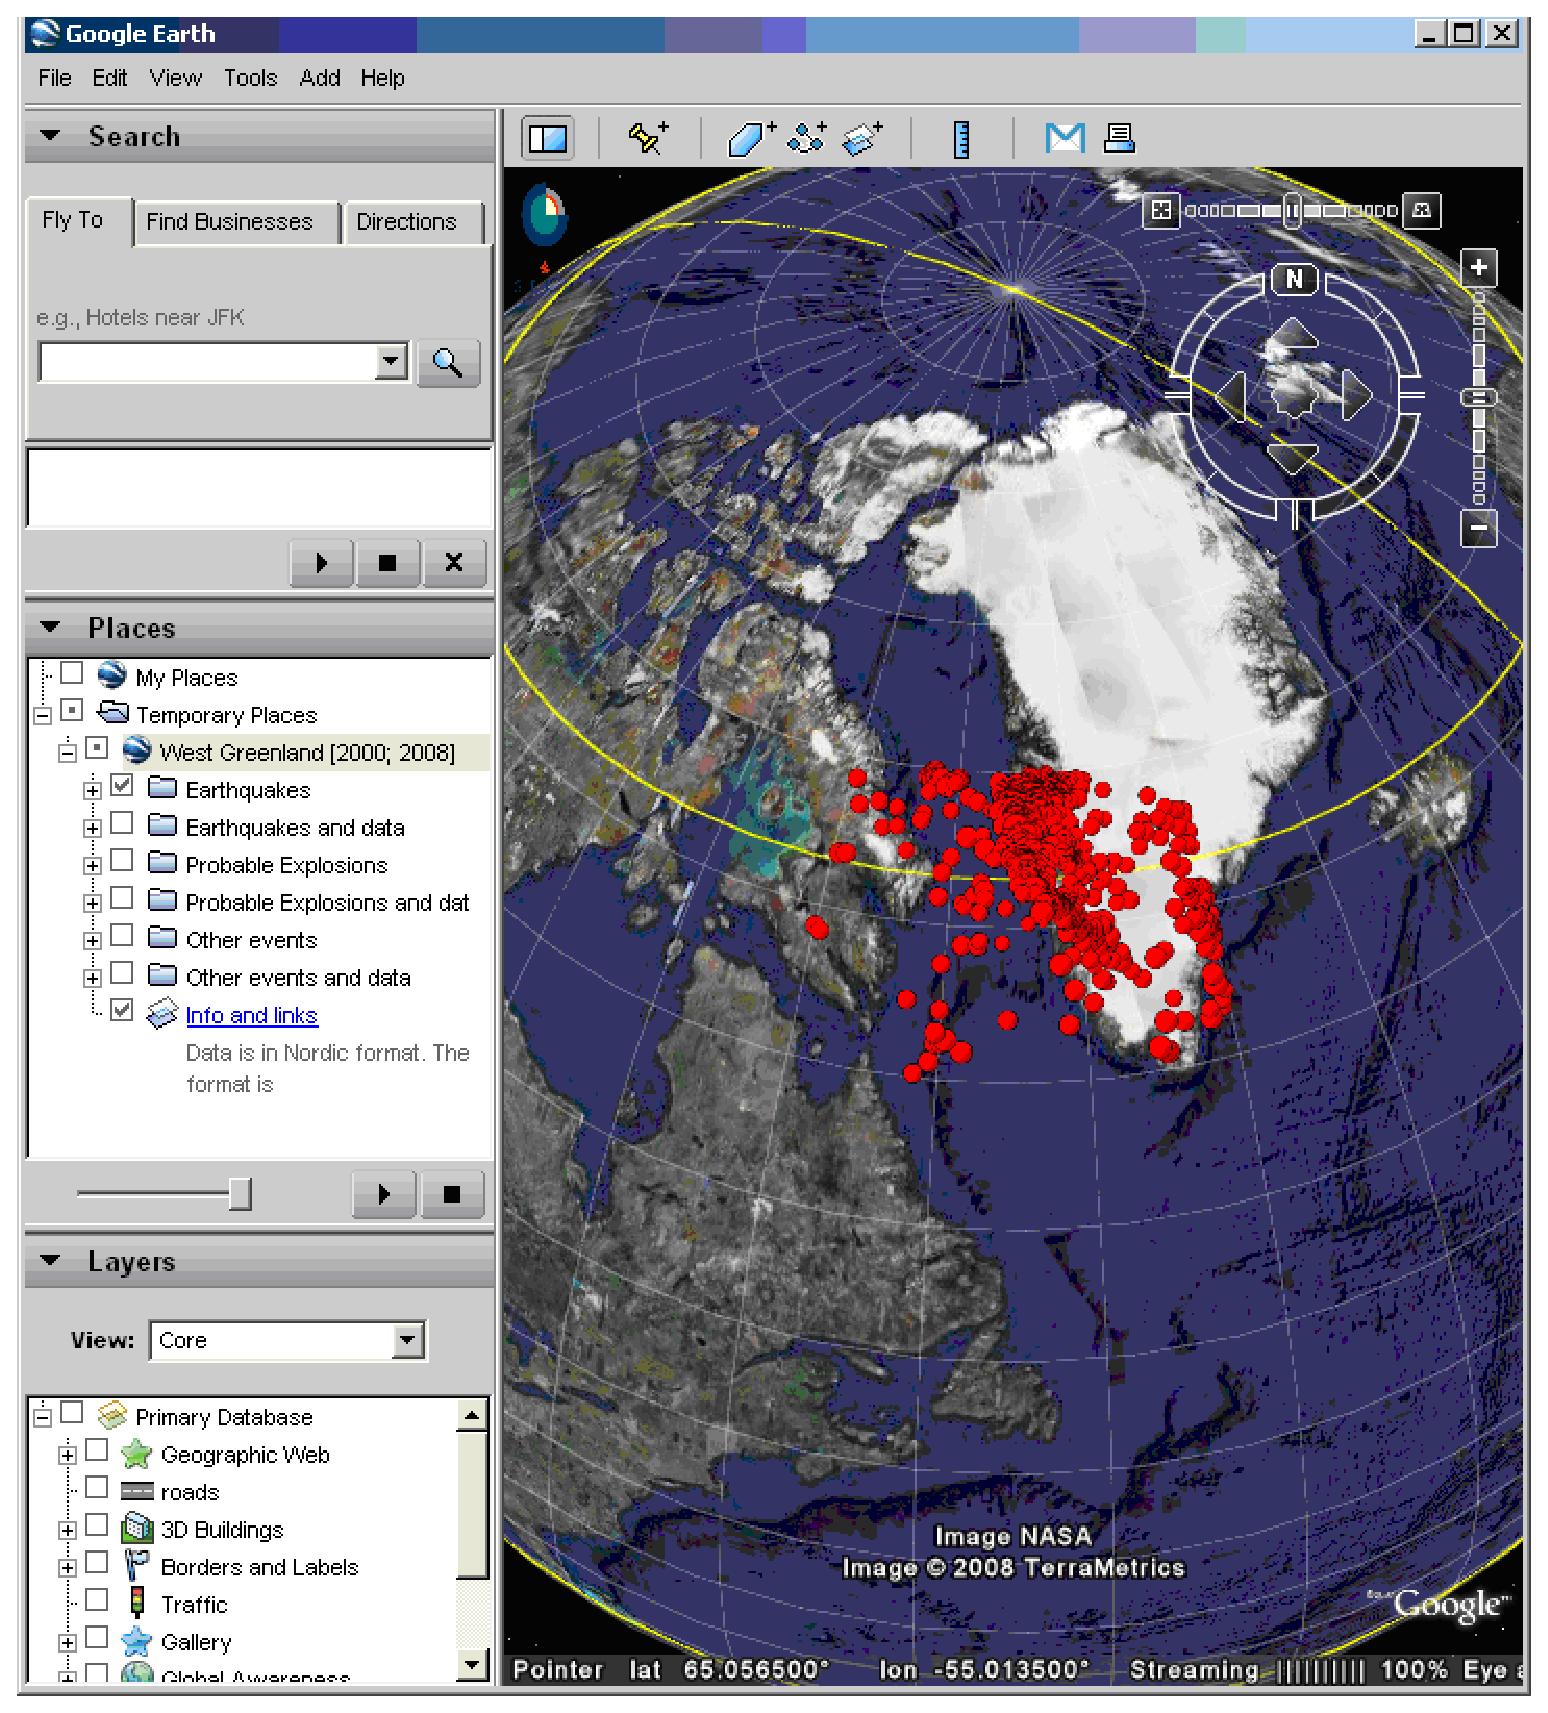
\includegraphics[width=0.9\linewidth]{fig/fig32}}
\caption{Example of mapping with gmap. Events in 
West Greenland. Note the folder and the subfolders in the \texttt{Places} window.}
\label{fig:gmap}
\end{figure}

To make an animation for events over time use the -timespan flag. As an example explosions in the south of Norway from 1983 to 2007 can be downloaded here: \url{http://seis.geus.net/ber-exp.kml} Press the play button at the time slider at the top of the Google Earth. Use the ruler to control how the animation is displayed (speed, days shown, etc.). 

\index{Raster file} 

\begin{figure}
\htmlimage{scale=2.0}
\centerline{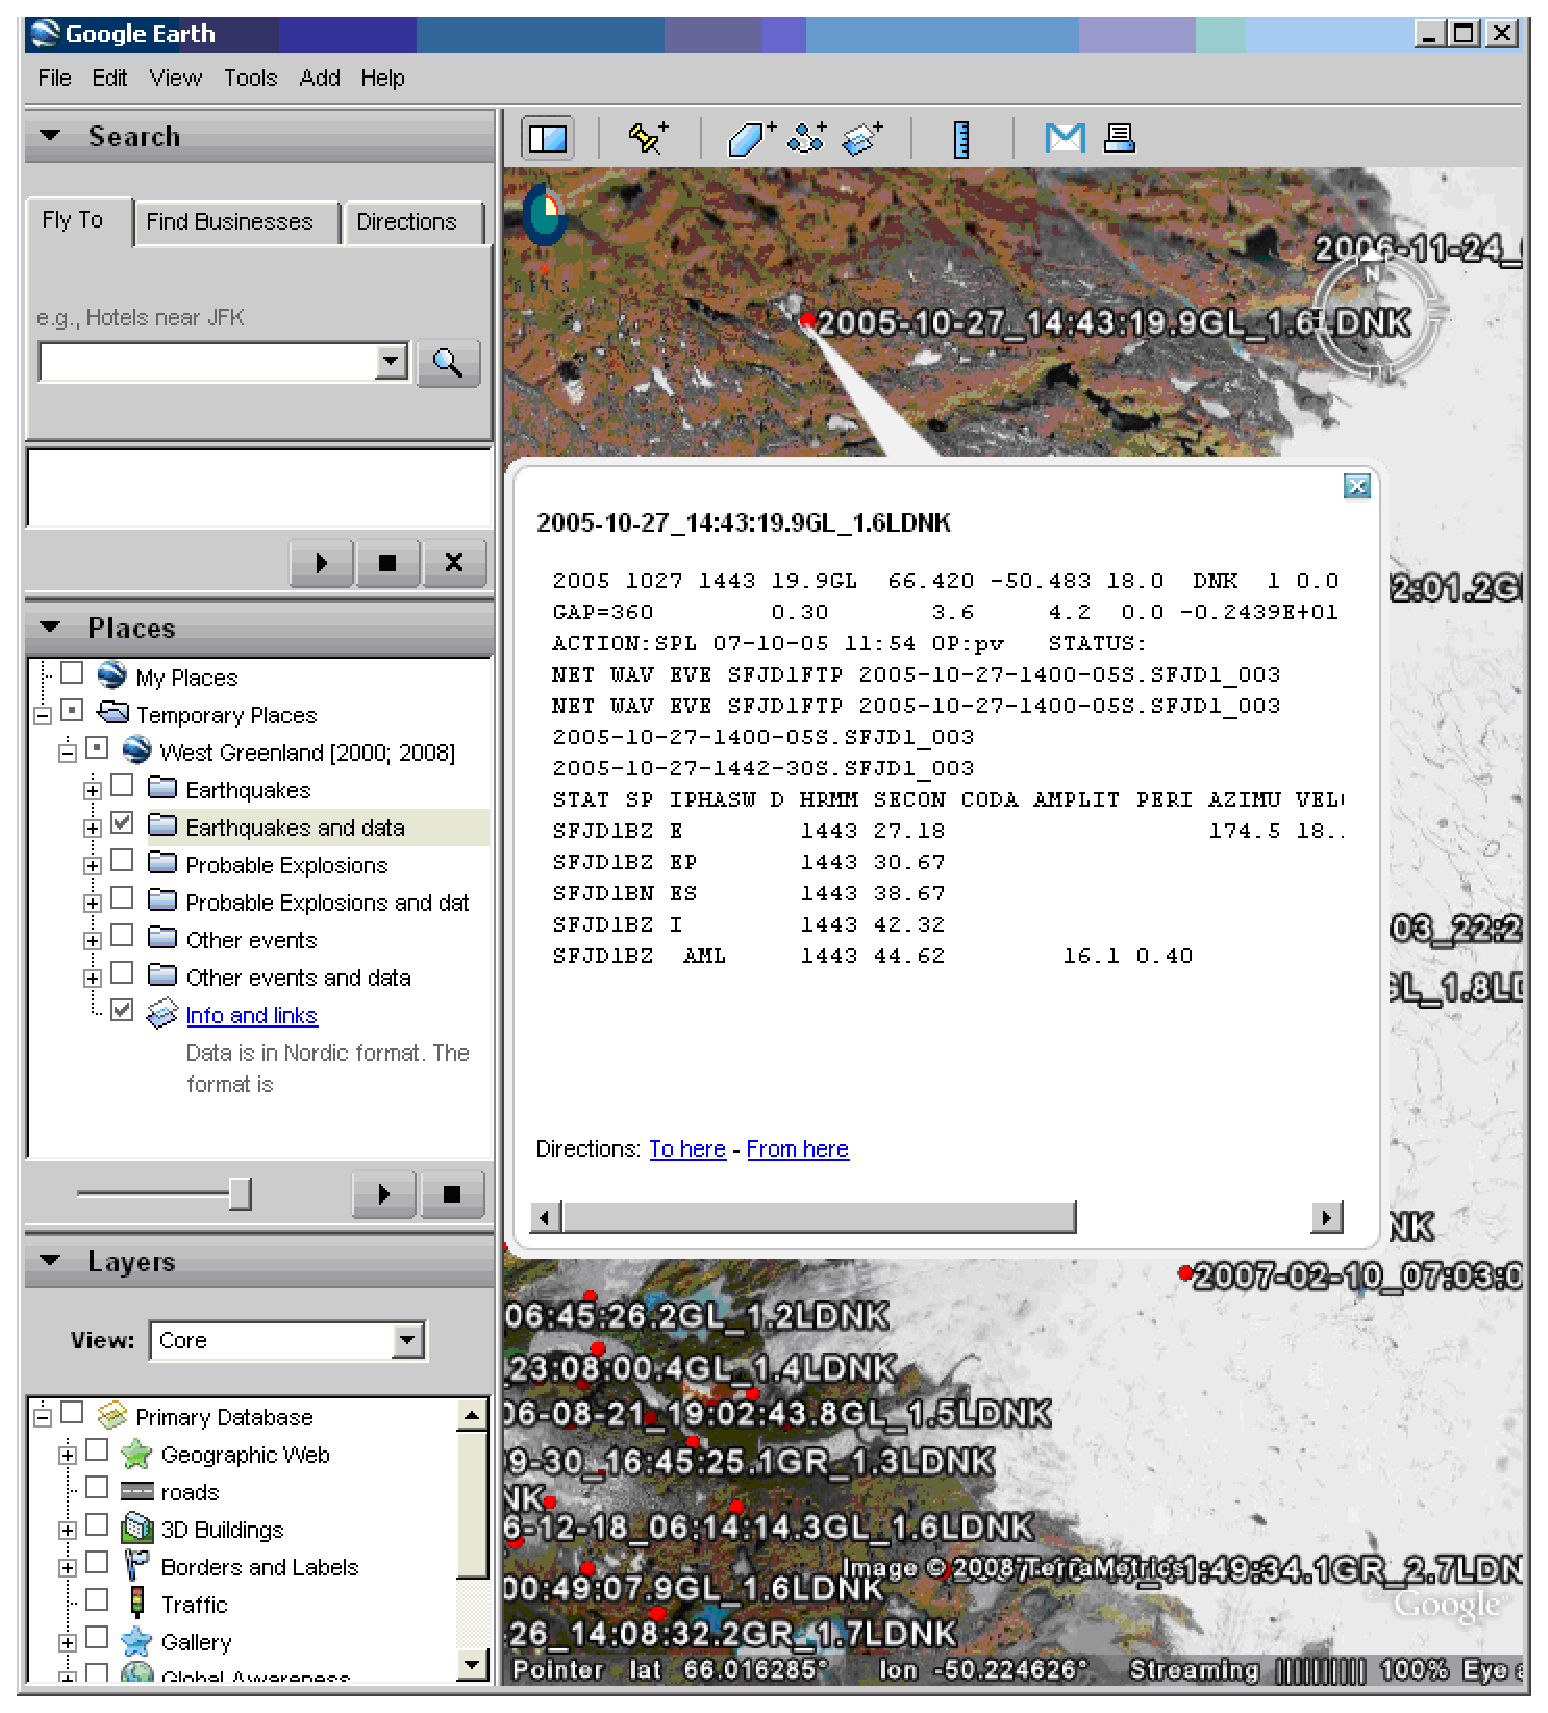
\includegraphics[width=0.9\linewidth]{fig/fig33}}
\caption{If the \texttt{Earthquakes and data} folder is selected in 
the \texttt{Places} window S-files can be shown.}
%\label{fig:}
\end{figure}

\begin{figure}
\htmlimage{scale=2.0}
\centerline{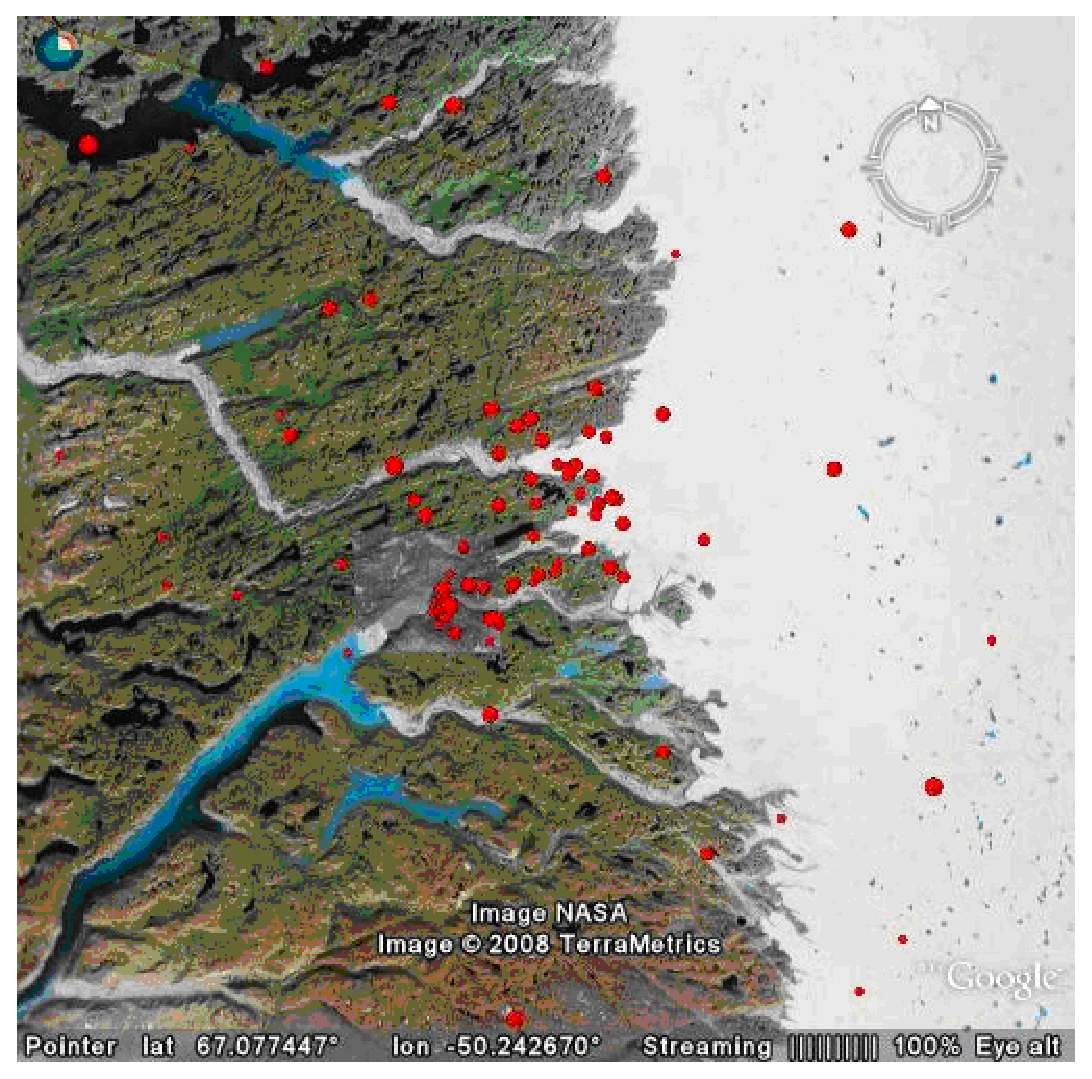
\includegraphics[width=0.9\linewidth]{fig/fig34}}
\caption{A map can be saved as raster file (File-Save-Save Image).}
%\label{fig:}
\end{figure}

GMAP parameters added to \texttt{SEISAN.DEF}: 
Icon used for earthquake, explosion, probable explosion and other events: 

\begin{small}
\verbatiminput{include/gmap.par.1}
\end{small}

Events with magnitude smaller than GMAP\_ICON\_MSIZE will be plottet with size of GMAP\_ICON\_MSIZE: 

\begin{small}
\verbatiminput{include/gmap.par.2}
\end{small}

The scale of the earthquake icons is give by GMAP\_ICON\_XSIZE*magnitude**GMAP\_ICON\_YSIZE: 

\begin{small}
\verbatiminput{include/gmap.par.3}
\end{small}

The scale of other events is furthermore multiplied by 2 Text can be added to the KML file, see this example, note the text must be placed from character no 41 to no 120: 

\begin{small}
\verbatiminput{include/gmap.par.4}
\end{small}

\textbf{GMAP -help:}

\begin{small}
\verbatiminput{include/gmap.help}
\end{small}

\subsubsection{The automatic GMAP}
\index{GMAP automatic} 

The automatic GMAP, is executed by the HYP program, when e.g. an event is located in EEV.

\begin{figure}
\htmlimage{scale=2.0}
\centerline{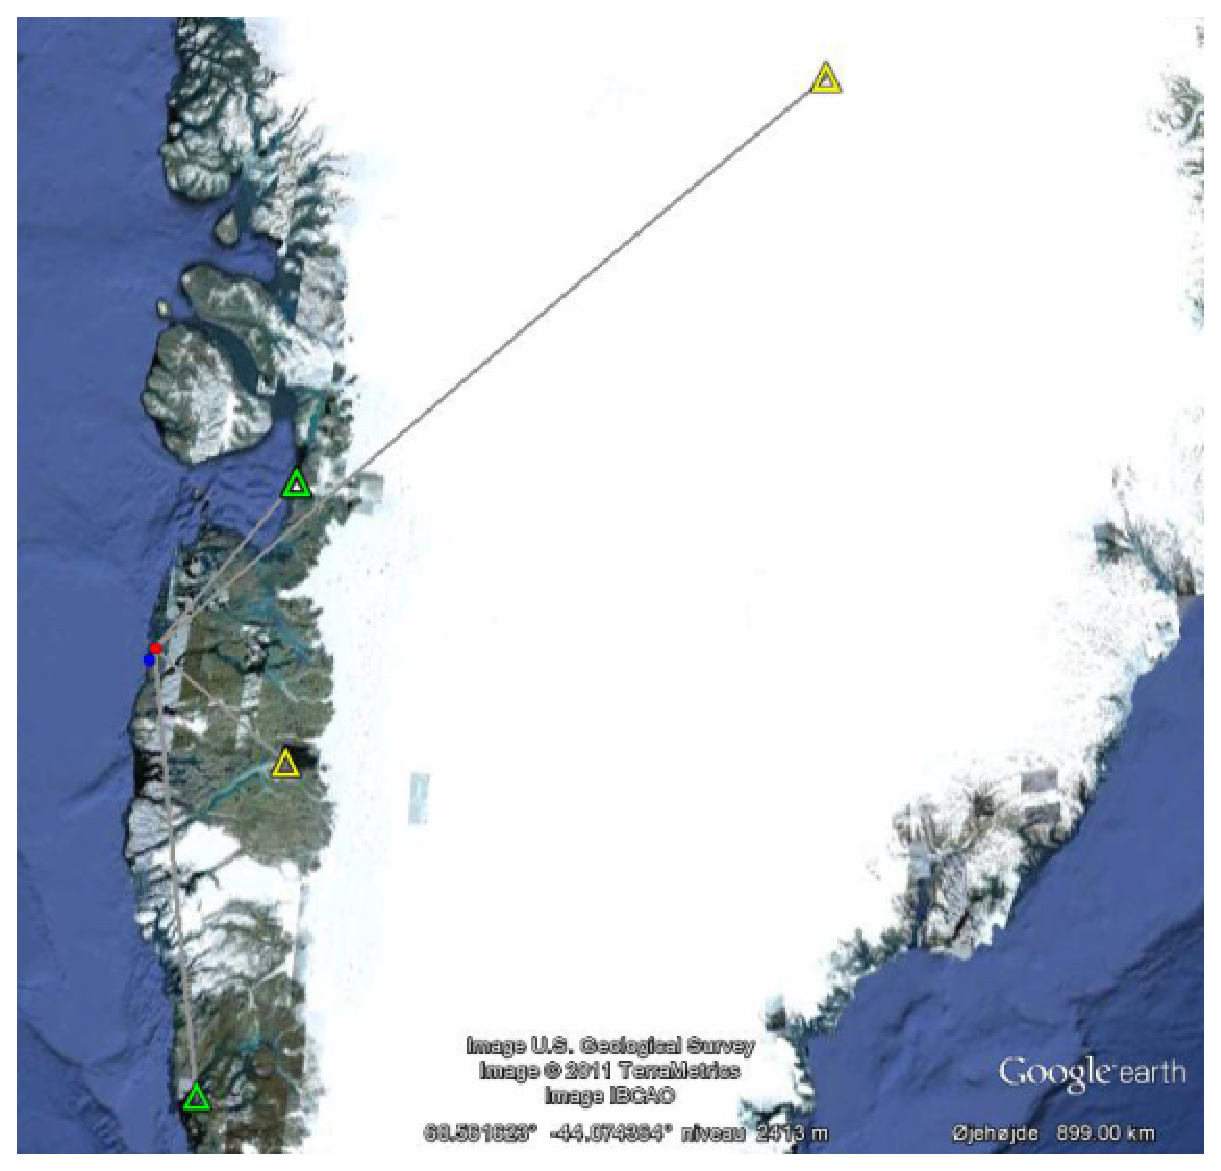
\includegraphics[width=0.9\linewidth]{fig/gmap-cur-kml}}
\caption{Example of automatic mapping with gmap. Earthquake in 
West Greenland. 
Blue dot is the old location and the red dot is the current location.
Green and yellow stations are stations with good and ok residuals, respectively.}
\label{fig:gmap.cur.kml}
\end{figure}

Start EEV and locate an event. In the directory a new file \texttt{gmap.cur.kml} 
will appear, this file can be opened with Google Earth and it will show 
the location of the current event and the used stations and the raypaths.

The color of the stations is given by the travel time residual as green, yellow or red,
for: residuals$<0.5s$, $0.5s=<$residual$=<1,5s$ or residual$>1.5s$, respectively.

To enable the automatic generation of Google Earth input files, add these parameters to your \texttt{SEISAN.DEF} file:

\begin{small}
\verbatiminput{include/gmap.par.5}
\end{small}

You can change the parameters to adjust the output file \texttt{gmap.cur.kml} for your system, see definition here \ref{ref:gmap.par}.

Inorder to run the display in a realtime mode, you must have an other KML file that makes Google Earth reload the \texttt{gmap.cur.kml} file at short intervals.
Such file could look like:

\begin{small}
\verbatiminput{include/gmap-automatic.kml}
\end{small}

In this example the \texttt{gmap.cur.kml} file is reloaded every 3 second from a local 
\texttt{C:\textbackslash seismo\textbackslash WOR} directory on a windows pc. 
And below is an other KML file is reloaded at 60min intervals from the Internet.

The above file is named \texttt{gmap-automatic.kml} and is found in the DAT directory.

